% Metódy inžinierskej práce

%\documentclass[10pt,twoside,slovak,a4paper]{article}
\documentclass{article}

\usepackage[slovak]{babel}
%\usepackage[T1]{fontenc}
\usepackage[IL2]{fontenc} % lepšia sadzba písmena Ľ než v T1
\usepackage[utf8]{inputenc}
\usepackage{graphicx}
\usepackage{url} % príkaz \url na formátovanie URL
\usepackage{hyperref} % odkazy v texte budú aktívne (pri niektorých triedach dokumentov spôsobuje posun textu)

\usepackage{cite}
%\usepackage{times}

\pagestyle{headings}

\title{Gamifikácia a jej aplikovanie v pracovnom prostredí\thanks{Semestrálny projekt v predmete Metódy inžinierskej práce, ak. rok 2022/2023, vedenie: Ing. Fedor Lehocki, PhD.}} % meno a priezvisko vyučujúceho na cvičeniach

\author{Dominik Teplan\\[2pt]
	{\small Slovenská technická univerzita v Bratislave}\\
	{\small Fakulta informatiky a informačných technológií}\\
	{\small \texttt{xteplan@stuba.sk}}
	}

\date{\small 30. október 2022} % upravte



\begin{document}

\maketitle

\begin{abstract}
Treba dopísať
\end{abstract}



\section{Úvod}

Motivujte čitateľa a vysvetlite, o čom píšete. Úvod sa väčšinou nedelí na časti.

%Uveďte explicitne štruktúru článku. Tu je nejaký príklad.
%Základný problém, ktorý bol naznačený v úvode, je podrobnejšie vysvetlený v časti~\ref{nejaka}.
%Dôležité súvislosti sú uvedené v častiach~\ref{dolezita} a~\ref{dolezitejsia}.
%Záverečné poznámky prináša časť~\ref{zaver}.

\section{Stav v skúmanej oblasti} \label{stav}

Počas skúmania mojej vybranej oblasti som zistil, že jej stav preskúmania odborníkmi a stav spracovania do odbornej literatúry je podľa môjho názoru podpriemerný. Myslím si, že je to kvôli tomu, že daná problematika je stále relatívne nová. Napriek tomu sa mi podarilo nájsť niekoľko článkov, ktoré som pozorne preštudoval, a na ktoré sa v mojom článku odkazujem. 

\subsection{Výsledky systematického prehľadu} 
Na danú tému sa mi podarilo nájsť starší ale veľmi podrobný systematický prehľad literatúry, ktorý mi umožnil získať aspoň približné čísla, ktoré môj názor potvrdzujú\cite{10.1007/978-3-319-56541-5_29}.Tento prehľad bol publikovaný v roku 2017 a zaoberal sa článkami, ktoré sa týkali gamifikácie v pracovnom prostredí. Podľa neho bolo na danú tému nájdených 586 článkov od roku 2005. Žiaľ iba 35 z nich bolo označených za relevantné články. Najstarší relevantný článok bol z roku 2011 čo opäť potvrdzuje môj názor, že ide o novú oblasť skúmania.

\section{Definície a pojmy} \label{definície}
\begin{itemize}
\item \textbf{Gamifikácia} Je proces vylepšovania služby
možnosťami pre herné zážitky s cieľom podporiť používateľovu
celkovú tvorbu hodnoty\cite{10.1145/2393132.2393137}. Môžem to definovať jednoduchšie ako implementáciu hry a herných prvkov ~\ref{prvky} do rôznych prostredí za účelom motivovania ľudí (v tomto prípade zamestnancov) a teda aj zlepšenia samotného (v tomto prípade pracovného) prostredia.
\item \textbf{Pracovné prostredie} V mojom článku budem veľmi všeobecne a veľmi jednoducho definovať pracovné prostredie ako akékoľvek prostredie, v ktorom prebieha práca vykonávaná ľudmi (zamestnancami).
\item (možno ďalšie pojmy, ktoré sa v mojom článku vyskytnú a budú potrebovať vysvetlenie)
\end{itemize}
%\input{}

%Z obr.~\ref{f:rozhod} je všetko jasné. 

\begin{figure*}[tbh]
\centering
%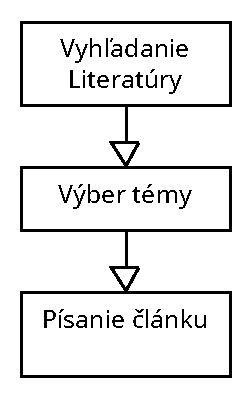
\includegraphics[scale=1.0]{Diagram.pdf}
%Aj text môže byť prezentovaný ako obrázok. Stane sa z neho označný plávajúci objekt. Po vytvorení diagramu zrušte znak \texttt{\%} pred príkazom %\verb|\includegraphics| označte tento riadok ako komentár (tiež pomocou znaku \texttt{\%}).
%\caption{Rozhodujúci argument.}
%\label{f:rozhod}
\end{figure*}

\section{Prvky gamifikácie a herné prvky} \label{prvky}

%Môže sa zdať, že problém vlastne nejestvuje\cite{Coplien:MPD}, ale bolo dokázané, že to tak nie je~\cite{Czarnecki:Staged, Czarnecki:Progress}. Napriek tomu, aj dnes na webe narazíme na všelijaké pochybné názory. Dôležité veci možno \emph{zdôrazniť kurzívou}.

Dôležitým aspektom úspešnej gamifikácie je výber herného dizajnu
prvkov. Prvky herného dizajnu určujú typ herných zážitkov
generovaných pre používateľov\cite{herne}. Inak povedané, je veľmi dôležité poznať a aplikovať do pracovného prostredia správne prvky hry, aby bol zamestnanec motivovaný a pracovitý. Týmto sa dosiahne nielen spokojnosť zamestnávateľov, ale aj samostných zamestnancov, pretože budú pracovať z vlastného záujmu. 

\subsection{Najčastejšie používané herné prvky} 
Všetky prvky by bolo zrejme nemožné vymenovať. Pokúsil som sa však zapísať a stručne vysvetliť aspoň tie najdôležitejšie a najčastejšie sa vyskytujúce herné prvky, ktoré sa pri gamifikácii využívajú.
\begin{itemize}
\item \textbf{Body} 
Sú to granulárne jednotky merania v gamifikácii. Toto je spôsob, akým systém uchováva počet akcií hráča, ktoré sa ho týkajú\cite{10.1007/978-3-642-39241-2_58}. Môžu fungovať aj ako herná mena, takže hráči ich môžu vymieňať za rôzne odmeny. Myslím si, že motivujúci faktor spočíva aj v zbieraní a hromadení týchto bodov.
\item \textbf{Rebríček}
Najjednoduchšie sa dá definovať ako zoznam hráčov (zamestnancov), v ktorom sa hráči môžu vzájomne porovnať a predbiehať. To znamená, že môže mať motivijúci, ale aj demotivujúci účinok.
\item \textbf{Cieľ}
Na to aby bola gamifikácia úspešná, je potrebné aby danú hru zamestnanci hrali čo najdlhšie a čo najviac. Najlepšie ako takéto niečo dosiahnuť je vytvoriť pre zamestnancov \textit{relevantný} cieľ, ktorý sa budú pokúšať dosiahnuť. Relevantným cieľom môže byť napríklad finančná odmena alebo posun vyššie v hierarchii pracovného prostredia.
\item \textbf{Pravidlá}
Podľa môjho názoru je to najdôležitejší prvok každej hry a teda aj gamifikácie. Ak nie sú presne definované pravidlá, tak vznikne chaos.
\\Pravidlá hry spájajú mechaniku do toku, aby motivovali hráča k dosiahnutiu cieľa\cite{10.1007/978-3-642-39241-2_58}.
\end{itemize}

\section{Dopad gamifikácie na pracovné prostredie} \label{dopad}




\section{Ešte dôležitejšia časť} \label{dolezitejsia}

\section{Pridaná sekcia}


\section{Záver} \label{zaver} % prípadne iný variant názvu



%\acknowledgement{Ak niekomu chcete poďakovať\ldots}


% týmto sa generuje zoznam literatúry z obsahu súboru literatura.bib podľa toho, na čo sa v článku odkazujete
\bibliography{Zdroj}
\bibliographystyle{abbrv} % prípadne alpha, abbrv alebo hociktorý iný
\end{document}
